\documentclass[journal, a4paper]{IEEEtran}
\usepackage[italian]{babel}
\usepackage{booktabs}
\usepackage{siunitx}%Questo serve a caricare il pacchetto delle unità di misura del sistema internazionale%
\usepackage[utf8]{inputenc}
\usepackage{graphicx} 
\usepackage{url}
\usepackage{amsmath}
\usepackage{amssymb}


\usepackage{keyval}
\usepackage{xcolor}
\usepackage{caption}
\usepackage{subfig}
\usepackage{tikz}
\usepackage{circuitikz}
\usepackage{authblk}
%\usepackage{hyperref}

\begin{document}


% Define document title and author
	\title{Tecnologie Digitali - Logbook Week 10}
	\author[1]{Salvatore Bottaro}
		\author[2]{Lorenzo M. Perrone}
		\affil[1]{\texttt{salvo.bottaro@hotmail.it}}
		\affil[2]{\texttt{lorenzo.perrone.lmp@gmail.com}}
	\markboth{Tecnologie Digitali - Di Lieto}{}
	\maketitle
	
\begin{abstract}
	Logbook di laboratorio di Tecnologie Digitali, a.a. 2015/2016. Week 10.
\end{abstract}

\section{Registri e circuiti logici sequenziali}

Un circuito logico sequenziale è un tipo di circuito logico in cui l'uscita non dipende solo dai valori degli ingressi ma anche dalla storia del circuito stesso. Pertanto essi devono essere costituiti da una parte che svolga la funzione di memoria, il circuito logico che svolga le operazioni, un segnale di \textit{clock} che funga da riferimento temporale.\\
Un registro o \textit{latch} è un dispositivo che svolge il ruolo di memoria. Il tipo più semplice è quello di tipo \textbf{SR}, ovvero \textit{SET-RESET}, in figura \ref{fig:sr}.

\begin{figure}[htp]
\centering
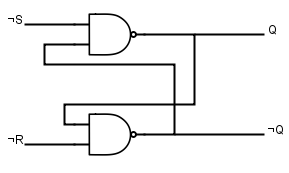
\includegraphics[scale=.5]{SR}
\caption{Schema di un registro SR.}
\label{fig:sr}
\end{figure}

\subsection{Hm. 1}

In tabella \ref{tab:sr} è data la tavola di verità del registro SR. Come si vede solo quando entrambi gli ingressi son veri le uscite non cambiano. Negli altri casi le uscite sono modificate indipendentemente dal loro valore iniziale.

\begin{table}[htp]
\centering
\caption{Tavola di verità del registro SR.}
\label{tab:sr}
\begin{tabular}{|c|c|c|c|}
\hline 
$\overline{S}$ & $\overline{R}$ & Q & $\overline{Q}$ \\ 
\hline 
T & T & Q & $\overline{Q}$ \\ 
\hline 
T & F & F & T \\ 
\hline 
F & T & T & F \\ 
\hline 
F & F & T & T \\ 
\hline 
\end{tabular} 
\end{table}

Per ovviare a questo si introduce un clock che funga da segnale di controllo, come in figura \ref{fig:latch}.

\begin{figure}[htp]
\centering
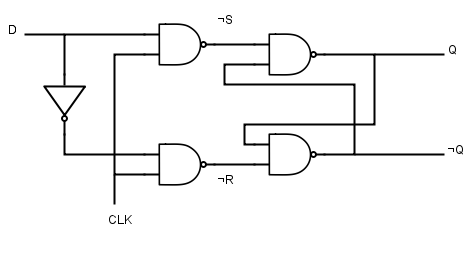
\includegraphics[scale=.4]{latch}
\caption{Registro SR con clock.}
\label{fig:latch}
\end{figure}

In tabella \ref{tab:latch} è data la tavola di verità del latch di tipo D, prendendo cme uscite gli ingressi del registro SR. Come si vede quando il clock è falso, gli ingressi del registro sono entrambi veri e le uscite sono conservate, quando il clock è vero, allora le uscite sono modificate. Pertanto per memorizzare le uscite basta tenere il clock sullo stato di falso.

\begin{table}[htp]
\centering
\caption{Tavola di verità latch di tipo D.}
\label{tab:latch}
\begin{tabular}{|c|c|c|c|}
\hline 
D & CLK & $\overline{R}$ & $\overline{S}$ \\ 
\hline 
T & T & F & T \\ 
\hline 
T & F & T & T \\ 
\hline 
F & T & T & F \\ 
\hline 
F & F & T & T \\ 
\hline 
\end{tabular} 
\end{table}

Quando il clock abilita il trasferimento del segnale di uscita (quindi quando è nello stato vero), lo stato dell'ingresso D può cambiare più volte, generando un'uscita imprevedibile.\\
I registri \textit{edge-triggered flip-flop} ovviano a questo problema consentendo le modifiche delle uscite solo nella fase di cambiamento dello stato del clock, quindi durante le fasi di salita o discesa del segnale. Il flip-flop impiegato in laboratorio è il 14013 della famiglia CMOS, dotati di due flip-flop edge-triggered. In figura \ref{fig:pinass} vi è la disposizione dei pin, mentre in figura \ref{fig:pindef} la funzione dei vari pin.

\begin{figure}[htp]
\centering
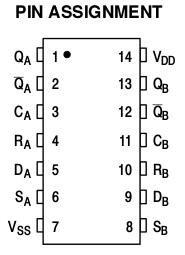
\includegraphics[scale=.4]{pinass}
\caption{Disposizione dei pin nel 14013}
\label{fig:pinass}
\end{figure}

\begin{figure}[htp]
\centering
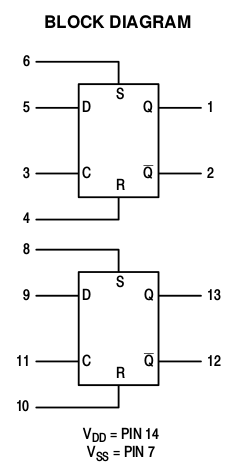
\includegraphics[scale=.4]{pindef}
\caption{Definizione dei pin.}
\label{fig:pindef}
\end{figure}

I tempi di risposta con i pin di S e R a terra (corrispondente alle modalità di lavoro in laboratorio) sono riassunti in figura \ref{fig:time}.

\begin{figure}[htp]
\centering
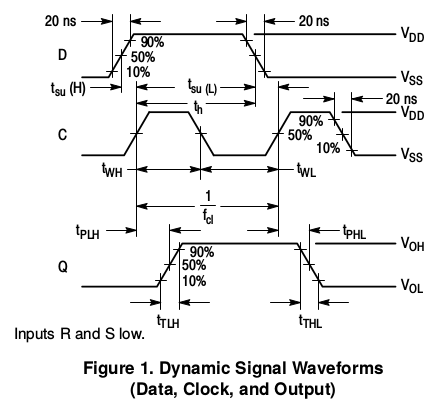
\includegraphics[scale=.4]{time}
\caption{Tempi di risposta con R e S a terra.}
\label{fig:time}
\end{figure}

Nelle tabelle \ref{tab:val} e \ref{tab:data} sono riassunti i valori di alcune grandezze caratteristiche rilevanti del 14013.

\begin{table}[htp]
\centering
\caption{Valori tipici del 14013.}
\label{tab:val}
\begin{tabular}{|c|c|}
\hline 
Grandezza & Valore \\ 
\hline 
Tensione di alimentazione & $V_{min} = -0.5 V$, $V_{max} = 18 V$ \\ 
\hline 
Input current & 10 mA \\ 
\hline 
Consumo massimo & 500 mW \\ 
\hline 
\end{tabular} 
\end{table}

\begin{table}[htp]
\centering
\caption{Fasce di tensione del 14013}
\label{tab:data}
\begin{tabular}{|c|c|c|}
  \hline
  Grandezza & $V_{DD}$ (V)& Valore \\
  \hline
           &  5  &  0.05 V \\ \cline{2-3}
  $V_{OL}$ & 10  &  0.05 V \\ \cline{2-3}
           & 15  &  0.05 V \\ 
  \hline 
           &  5  &  4.95 V \\ \cline{2-3}
  $V_{OH}$ & 10  &  9.95 V \\ \cline{2-3}
           & 15  & 14.95 V \\ 
  \hline \hline
           &  5  &  1.5 V \\ \cline{2-3}
  $V_{IL}$ & 10  &  3.0 V \\ \cline{2-3}
           & 15  &  4.0 V \\ 
  \hline 
           &  5  &  3.5 V \\ \cline{2-3}
  $V_{IH}$ & 10  &  7.0 V \\ \cline{2-3}
           & 15  &   11 V \\ 
  \hline
\end{tabular}
\end{table}

\subsection{Hm. 2}

In figura \ref{fig:truth} è mostrata la tavola di verità del 14013. Come si vede solo quando il segnale di clock decresce le uscite risultano conservate, negli altri casi dipende dal valore degli ingressi D, R, S (in particolare a noi interessano i casi R=S=0).

\begin{figure}[htp]
\centering
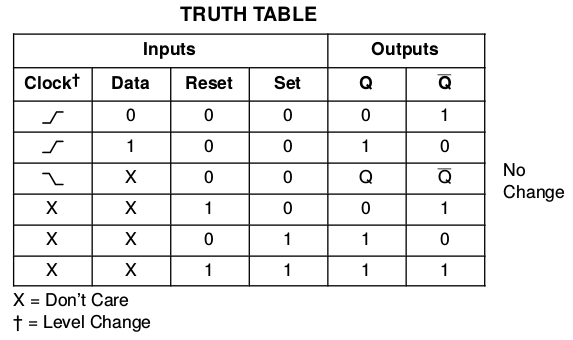
\includegraphics[scale=.4]{truth}
\caption{Tavola di verità del 14013.}
\label{fig:truth}
\end{figure}

\subsection{Hm. 3}

Nel datasheet è indicata una possibile applicazione del 14013, della \textit{n-stage shift register} in figura \ref{fig:shift}.

\begin{figure}[htp]
\centering
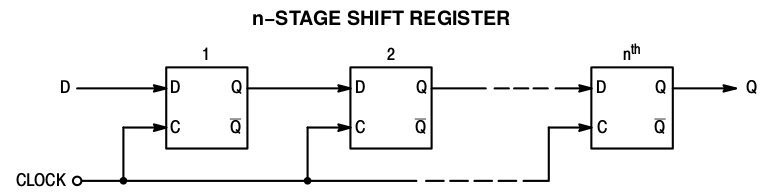
\includegraphics[scale=.3]{shift}
\caption{Schema dello shift register}
\label{fig:shift}
\end{figure}

Calcolando la tavola di verità si vede che il valore di Q coincide con quello di D iniziale, per cui la funzione di questo dispositivo potrebbe essere quello di spostare il valore di una variabile (in questo caso D) da una certa allocazione nella memoria ad un'altra distante n-1 "passi".

\section{contatori}

Una funzione degli edge-triggered flip-flop è quella di contatore asincrono, ovvero divisori di frequenza. In figura \ref{fig:div} è mostrato lo schema di un divisore per 2.

\begin{figure}[htp]
\centering
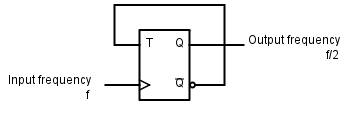
\includegraphics[scale=.6]{contatore}
\caption{Schema di un divisore per 2.}
\label{fig:div}
\end{figure}

Per calcolare la tavola di verità bisogna trasferire il valore di $\overline{Q}$ nella colonna dei valori di D, dopodiché calcolare il nuovo valore di Q e $\overline{Q}$ in base alla variazione del clock. Si ottiene così la tabella \ref{tab:tabdiv} in cui si vede come un periodo di Q (la sequenza 0011) contiene due periodi del clock, ovvero il segnale in uscita ha una frequenza pari a metà di quella del clock.

\begin{table}[htp]
\centering
\caption{Tavola di verità del divisore per 2.}
\label{tab:tabdiv}
\begin{tabular}{|c|c|c|c|}
\hline 
CLK & D & $\overline{Q}$ & Q \\ 
\hline 
X & X & 0 & 1 \\ 
\hline 
$\uparrow$ & 0 & 1 & 0 \\ 
\hline 
$\downarrow$ & 1 & 1 & 0 \\ 
\hline 
$\uparrow$ & 1 & 0 & 1 \\ 
\hline 
$\downarrow$ & 0 & 0 & 1 \\ 
\hline 
$\uparrow$ & 0 & 1 & 0 \\ 
\hline 
\end{tabular} 
\end{table}

Abbiamo verificato il funzionamento del divisore realizzando sulla breadboard lo schema \ref{fig:div} e collegato all'uscita il tester digitale. Il segnale di clock è stato prodotto tramite il VI \texttt{Digital$\_$out4} ed effettivamente abbiamo ritrovato la tavola di verità prevista.

Successivamente abbiamo impiegato un generatore di segnale come segnale di clock, impostando una frequenza di circa 25 kHz. Tramite il VI \texttt{Contatore$\_$freq} abbiamo verificato la stabilità in frequenza del segnale. In tabella \ref{tab:freq} sono riassunti i risultati dell'istogramma fornito dal VI, su 500 campionamenti effettuati.

\begin{table}[htp]
\centering
\caption{Campionamento in frequenza del segnale emesso dal generatore.}
\label{tab:freq}
\begin{tabular}{|c|c|}
\hline 
Frequenza (kHz) & n \\ 
\hline 
25.708 & 17 \\ 
\hline 
25.738 & 438 \\ 
\hline 
25.771 & 45 \\ 
\hline 
\end{tabular}
\end{table} 

La frequenza rilevata risulta essere 25.740(11) kHz, effettuando diverse prove non abbiamo notato variazioni significative nella frequenza rilevata, con differenze dell'ordine dei 10-20 Hz. Abbiamo inoltre verificato che la misura del periodo del segnale effettuata dal VI corrispondesse all'inverso della frequenza misurata.\\
Abbiamo quindi collegato l'uscita del divisore alla scheda e avviato l'acquisizione. I risultati sono riassunti in tabella \ref{tab:div}. Risulta evidente che la frequenza in uscita é metà di quella in ingresso e che quindi il comportamento del dispositivo è ben verificato in questa modalità.

\begin{table}[htp]
\centering
\caption{Campionamento in frequenza del segnale in uscita dal divisore.}
\label{tab:div}
\begin{tabular}{|c|c|}
\hline 
Frequenza (kHz) & n \\ 
\hline 
12.878 & 345 \\ 
\hline 
12.886 & 155 \\ 
\hline 
\end{tabular} 
\end{table}

Collegando in serie più divisori per 2 è possibile costruire dei divisori per $2^n$, come si può ricavare dal datasheet. In figura \ref{fig:divider} lo schema del divisore per $2^n$ ricavabile dal datasheet.

\begin{figure}[htp]
\centering
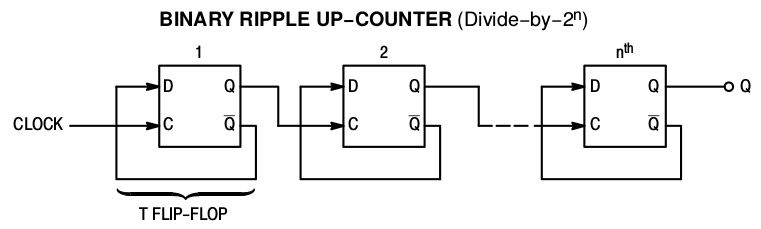
\includegraphics[scale=.3]{divider}
\caption{Schema di un divisore per $2^n$.}
\label{fig:divider}
\end{figure}

Abbiamo realizzato nello specifico un divisore per 4, quindi lo schema in figura \ref{fig:div4}.

\begin{figure}[htp]
\centering
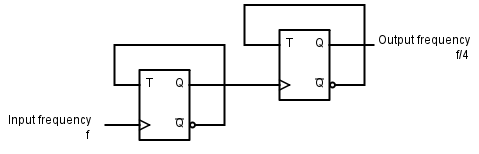
\includegraphics[scale=.4]{divider4}
\caption{Schema del divisore per 4.}
\label{fig:div4}
\end{figure}

In tabella \ref{tab:4} è mostrata la tavola di verità del divisoe per 4. Come si vede il periodo dell'uscita Q2 è 4 volte il periodo del clock, per cui la frequenza del segnale in uscita ha frequenza pari a $\frac{1}{4}$ della frequenza di ingresso.

\begin{table}[htp]
\centering
\caption{Tavola di verità del divisore per 4.}
\label{tab:4}
\begin{tabular}{|c|c|c|c|c|c|c|c|}
\hline 
CLK1 & D1 & $\overline{Q1}$ & Q1 & CLK2 & D2 & $\overline{Q2}$ & Q2 \\ 
\hline 
X & X & 0 & 1 & X & X & 0 & 1 \\ 
\hline 
$\uparrow$ & 0 & 1 & 0 & $\downarrow$ & 0 & 0 & 1 \\ 
\hline 
$\downarrow$ & 1 & 1 & 0 & - & 0 & 0 & 1 \\ 
\hline 
$\uparrow$ & 1 & 0 & 1 & $\uparrow$ & 0 & 1 & 0 \\ 
\hline 
$\downarrow$ & 0& 0 & 1 & - & 1 & 1 & 0 \\ 
\hline 
$\uparrow$ & 0 & 1 & 0 & $\downarrow$ & 1 & 1 & 0 \\ 
\hline 
$\downarrow$ & 1 & 1 & 0 & - & 1 & 1 & 0 \\ 
\hline 
$\uparrow$ & 1 & 0 & 1 & $\uparrow$ & 1 & 0 & 01\\ 
\hline 
$\downarrow$ & 0 & 0 & 1 & - & 0 & 0 & 1 \\ 
\hline
\end{tabular} 
\end{table}

Impiegando come segnale di clock il segnale a 25 kHz del generatore, tramite il VI \texttt{Contatore$\_$freq} abbiamo ottenuto i risultati di tabella \ref{tab:div4}, da cui si evince che la frequenza di uscita è pari a $\frac{1}{4}$ la frequenza di ingresso.

\begin{table}[htp]
\centering
\caption{Campionamento in frequenza del segnale in uscita dal divisore.}
\label{tab:div4}
\begin{tabular}{|c|c|}
\hline 
Frequenza (kHz) & n \\ 
\hline 
6.444 & 498 \\ 
\hline 
6.506 & 2 \\ 
\hline 
\end{tabular} 
\end{table}

\end{document}